\subsubsection{PHP (Handle)}
Die Abkürzung PHP steht für "PHP Hypertext Preprocessor". Es handelt sich hierbei um ein serverseitige Programmiersprache, die vor allem in der Webentwicklung zum Einsatz kommt. Die Syntax ist an Perl und C angelehnt.\\
Als PHP-Module wurden nur php5-mysql sowie php5-ldap verwendet.\\
PHP ist seit Version 5 vollständig Objekt-orientiert, wurde aber imperativ/funktional verwendet.\\
\\
Ein PHP Programm kann im Gegensatz zu anderen serverseitigen Programmiersprachen direkt in den HTML-Quelltext der Website eingebunden werden. Gekennzeichnet werden diese eingebetteten Programme mit den PHP-Tags (siehe Programm-Code 3.1).\\
\begin{lstlisting}[style=customPHP, caption={PHP-Tags}]
<?php 
	/* Programm-Code */
?>
\end{lstlisting}
Befindet sich der PHP Code eingebettet in HTML-Quelltext, so ignoriert der Interpreter alles, das außerhalb der PHP-Tags steht.\\\\
Eines der großen Vorteile an PHP ist, dass es vollständig serverseitig verarbeitet wird, das heißt am Client wird keine Rechenleistung für das Ausführen des PHP-Codes benötigt.
\paragraph{Funktionsweise}
Der Client fragt am Webserver eine Datei mit der Endung .php an. Anschließend lädt der Webserver die Datei und übergibt diese dem PHP Interpreter. Dieser generiert in den meisten Fällen eine HTML Datei, welche anschließend dem Webserver übergeben wird. Dieser sendet die "fertige" Webseite an den Client. (siehe Abb. 3.3) Der PHP Interpreter ist nicht nur auf HTML Dateien begrenzt, es können auch andere Dateitypen, wie Bilder oder PDF Dateien generiert werden. Diese Funktionsweise hat das Problem, dass die Seite bei jedem neuen Aufruf erneut generiert werden muss, dies führt zu einer höheren Auslastung am Webserver. Um dieses Problem zu vermindern gibt es die Caches am Webserver, die häufig verwendete Programmteile zwischenspeichern, um sie bei erneutem Aufruf nicht erneut Compilieren zu müssen.
\begin{figure}[H]
\centering
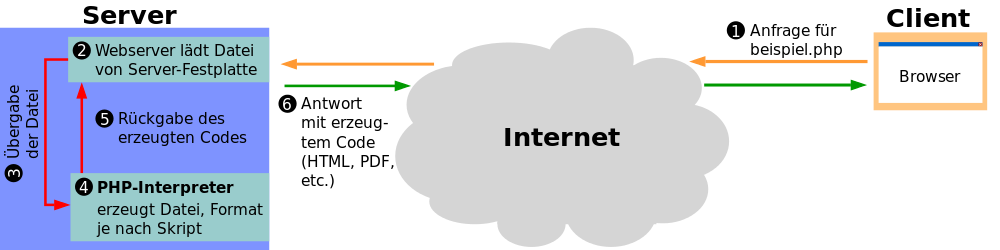
\includegraphics[keepaspectratio=true, width=14cm]{images/PHP_Funktionsweise.png}
\label{Abb 3.3}
\caption{PHP Funktionsweise}
\end{figure}
\paragraph{PHP Sessions}
Mit PHP Sessions kann man einen Besucher einer Webseite über mehrere Aufrufe der Webseite hinweg genau identifizieren. Jedem Besucher auf der Webseite wird eine eindeutige Session-ID zugewiesen, diese wird in einem Cookie auf dem Server abgelegt. Eine PHP Seite die die Session verwenden soll, muss als erstes des PHP-Dokuments diese Zeile stehen. (siehe Programm-Code 3.2)
\begin{lstlisting}[style=customPHP, caption={Session}]
<?php
	session_start();
?>
\end{lstlisting}

Damit wird dem Webserver vermittelt, dass diese Seite mit einer Session arbeitet.\\
Die session-ID ist eine 128 Bit lange Zahl die zufällig generiert wird. Diese muss ab nun bei jeder Antwort vom Server an den Client mitgeliefert werden und auch umgedreht. Damit können personenbezogene Informationen einer bestimmten Person zugewiesen werden, wie ein Warenkorb bei Online-Shopping, Status von einer Anmeldung usw. Wir verwenden Sessions um den User über die Webseite hinweg identifizieren zu können. 
\paragraph{Kommunikation mit Server}
PHP hat auch eine Möglichkeit, um diverse Daten dem Server zu 
senden, diese können von der zu empfangenden Webseite verarbeitet werden.\\\\
Diese Funktion wird vor allem bei Formularen eingesetzt, um die User-Interaktion mit der Seite zu steuern. Es wird auch dazu verwendet um auf einer Seite zu navigieren oder ein Login bereitzustellen. Jedoch muss man im Bereich im wesentlichen in 2 Teile unterteilen:
\begin{itemize}
    \item POST
    \item GET
\end{itemize}
\subparagraph{POST}
Bei POST werden die mitgegebenen Daten nicht an die URL angefügt, wie bei GET, aber dazu später, sondern werden im Body Teil der HTTP/S Anfrage an den Server. (siehe Programm-Code //TODO??) Dies hat den großen Vorteil, dass die mitgegebenen Daten praktisch eine unbegrenzte Größe haben können. Dadurch können auch lange Texte, Bilder, Dateien usw. an den Server gesendet werden. Ein weiterer Vorteil liegt darin, dass der User die eingegebenen Daten nicht sieht, d.h. gibt er ein Passwort ein so ist es für ihn nicht einsehbar. Dies schützt jedoch nicht vor Angreifer, die die HTTP Anfragen mitschneiden, deshalb verwendet man bei senden von Passwörtern immer HTTPS.\\
Im Beispiel Programm-Code ?? ist ein kleine Eingabe von einem Text möglich. Bei drücken des Buttons Speichern wird an den Server eine Anfrage gestellt, dass die gleiche Seite nochmals aufgerufen werden sollte, jedoch werden POST Variablen mitgegeben. Diese wertet die Seite mit dem PHP Teil aus und gibt den eingegebenen Text aus. Da dieser Text beliebig lang sein kann, muss POST verwendet werden. Warm siehe Punkt GET.
\begin{lstlisting}[style=CustomPHP, caption={Ausschnitt HTTP-Body}]
GET /login/index.php	//Angefragte Seite
HOST sis.htlinn.ac.at	//Host
.	//Weitere Informationen
.	//Weitere Informationen
.	//Weitere Informationen
user=20091234&password=passwort&send=1	//POST-Parameter
\end{lstlisting}
\begin{lstlisting}[style=CustomPHP, caption={Beispiel POST}]
<html>
<header>
</header>
<body>
<?php

if(!empty($_POST['text']))	//Wenn die Variable text nicht leer ist
	echo $_POST['text'];	//Soll der Text ausgegeben werden
else	//Wenn sie leer ist
	echo "nichts eingegeben";	//Soll eine Warnung ausgegeben werden
?>

<form method="post">	//method="post" --> Parameter werden mit POST mitgegeben
	<textarea name="text"></textarea>
	<button type="submit" name="save" value="Speichern">
</form>
</body>
</html>
\end{lstlisting}
\subparagraph{GET}
Bei GET werden die mitgegebenen Parameter direkt an die URL angehängt, um dies trennen zu können, wird die Parameterliste mit einem ? eingeleitet. Einzelne Parameter werden mit einem \& getrennt. Diese Methode ist die Standardmethode wenn man ein HTML-Form erstellt. Dies wird bei kleinen Daten verwendet. Der Vorteil liegt darin, dass der User die Seite neu laden kann und die Parameter werden übernommen. Auch kann der User die URL samt den Parametern als Lesezeichen abspeichern, um beispielsweise bei einer Webseite, die die Parameter zur Navigation auf der Seite verwendet, genau die gewünschte Seite zu erhalten. Eine Beispiel-URL sieht wie folgt aus: \textit{sis.htlinn.ac.at/index.php?text=hallo\&send=Speichern}. Dies wäre die URL, die bei absenden des Beispiel Programm-Codes ?? entstehen würde. Sofern die Datei des Programm-Codes index.php heißt. Im Prinzip läuft die Auswertung der mitgelieferten Parametern gleich ab, wie bei POST Parametern.\\
Bei GET besteht die Grenze der Datenlänge darin, dass eine URL nur ca. 2000 lang sein darf, dies ist Browser und Server abhängig, aber 2000 Zeichen funktioniert bei allen Server-Client Kombinationen.
\begin{lstlisting}[style=CustomPHP, caption={Beispiel GET}]
<html>
<header>
</header>
<body>
<?php

if(!empty($_GET['text']))	//Wenn die Variable text nicht leer ist
	echo $_GET['text'];	//Soll der Text ausgegeben werden
else	//Wenn sie leer ist
	echo "nichts eingegeben";	//Soll eine Warnung ausgegeben werden
?>

<form method="get">	//method="get" --> Parameter werden mit GET mitgegeben
	<input type="text" name="text"></textarea>
	<button type="submit" name="save" value="Speichern">
</form>
</body>
</html>
\end{lstlisting}
\paragraph{Probleme}
\subparagraph{Typisierung} 
Die Typisierung in PHP ist sehr flexible (dynamisch), so kann einer Variable, die zum Beispiel eine Zahl enthält, eine Zeichenkette, oder ein Array neu zugewiesen werden.\\
Manche Standard-Funktionen in PHP haben numerische Rückgabewerte und geben den bool'schen Wert false zurück, wenn ein Fehler auftritt. Da alle Werte, die nicht 0 sind, laut Definition gleich dem bool'schen true sind, kann es zu Fehlinterpretation des Rückgabewertes kommen. Um solche Situationen so vermeiden, sollte statt auf Wertegleichheit (==) auf Äquivalenz (===), das bedeutet in diesem Zusammenhang Werte- und Typgleichheit (Bool != Integer, trotz dynamischer Typisierung), geprüft werden (Beispiel: siehe Programm-Code ??).
\begin{lstlisting}[style=customPHP, caption={false}]
<?php 
	$string = "Hallo Welt";
	$position = strpos("H", $string); 
	// H liegt an Position 0
	
	// falsch:
	if ($position == false) {
		echo "Abfrage 1\n";
	}
	// richtig:
		if ($position === false) {
		echo "Abfrage 2\n";
	}
?>
\end{lstlisting}
\subparagraph{Serverseitige Realisierung}
Ein Problem und gleichzeitig auch ein Vorteil besteht darin, dass der Webserver die PHP-Datei compiliert und eine fertige HTML-Datei an den Client sendet. Der Vorteil liegt darin, dass keine Rechenleistung am Client nötig ist. Jedoch bedeutet dies auch, dass ohne neue Anfrage zum Server und daraus resultierendes Neu Laden der ganzen Seite kann sich nichts am Seitenaufbau ändern. Soll sich z.B. bei Auswählen einer Check Box etwas am Aufbau der Seite ändern, so muss entweder die Seite neu geladen werden oder man greift auf Technologien wie Ajax oder Java Script zurück.\\
Bei Java Script kann man bestimmte Eigenschaften abändern oder neue Objekte erstellen usw. (Siehe Punkt 3.1.4.2)\\
Bei Ajax wird prinzipiell eine neue Abfrage an den Server gestellt, also eine PHP Seite wird aufgerufen und die Antwort wird in die bestehende Seite eingebaut. (Siehe Punkt 3.1.4.3)\\